\chapter{Methodology}
\label{chap:deploymenttool}
todo: Downlink traffic is created by modulation of frequencies caused by a base station. However, 
 
\section{Calculating downlink exposure}
\subsection{Calculating exposure towards a single femtocell}
\label{sec:calculatingexposure}
To determine the total exposure of a single human being or even of the entire network, the electric-field $\vec{E}$ of a single femtocell $i$ should be calculated.
The formula to determine this electromagnetic value $E$ (expressed in V/m) for a specific location is given in equation \ref{eq:singleexposure}.
\begin{equation}
E_i = 10^{\frac{EIRP - 43.15 + 20*\log(f)- PL}{20}}
\label{eq:singleexposure}
\end{equation}
This formula requires several values to be known. The frequency $f$ on which the tranmitting antenna is operating is expressed in MHz. The other values are explained in \ref{subsec:eirp} and \ref{subsec:pl}.

\subsubsection{EIRP}
\label{subsec:eirp}
A directional antenna can achieve gain by focussing it's input power into certain directions. By doing this, some areas experience a decreased radiation power in order to gain radiation power 
in the other privileged areas. If a theorical \gls{isotropicradiator} existed, the \gls{EIRP} is the power it would require to achieve the same power level as the actual antenna's main lob. The main lob is the area of the directional antenna experiencing the most gain.
This \gls{EIRP} value can be calulated as described in eq \ref{eq:eirp}.
\begin{equation}
EIRP = P_t + G_t - L_t
\label{eq:eirp}
\end{equation}

This value is expressed in dBm and requires tree values. $P_t$ is the transmit power (dBm), $G_t$ is the gain (dBi) of the transmitting antenna and $L_t$ stands for it's cable loss (dB) \cite{howToCalculateEIRP}.

\subsubsection{PL}
\label{subsec:pl}
At last, formula \ref{eq:eirp} requires the path loss (dB). In order calculate the path loss, an appropiate propagation model is required. Several propagation models exists and the tool already uses the Walfish-Ikegami model \cite{J2}.
This is because the Walfish-Ikegami model performs well for femtocell networks in urban areas. %optioneel kan je hier dezelfde bron gebruiken als dat ze in thesis van de vorige gebruikten. Bron nummer 32
The chosen propagation model consists of two formulas depending on whether a free line of sight between the user and the basestation exist or not. Both formulas expect a distance in kilometer. %bron?

input power hangt af van bs tot bs.

\subsection{Combining exposure}
\label{sec:combiningexposure}
manets -> exosure combineren
\begin{equation}
E_{tot} = \sqrt{\sum_{i=1}^{n} E_i^2}
\label{eq:totalexposure}
\end{equation}




%\section{Radiation Patterns}
%\label{sec:radiationpatterns}
%When approaching an antenna as an \gls{isotropicradiator}, gain is distributed equally in all directions. This is however only a theoretical antenna. In real life, an antenna's gain is restricted to a limited area.
%Therefore, a negative attenuation value should be added to the formula in order to compensate for the generalization of equal distributed gain \cite{AttenuationSectorizationForHSPA, AttenuationSystemLevelanalyssis}.
%Am=25dB 
%\begin{equation}
%A(\varphi)=-\min\left[12\left({\varphi\over \varphi_{3dB}}\right),A_{m}\right]
%\end{equation}

%SLA=20dB
%\begin{equation}
% A(\theta)=-\min\left[12\left({\theta\over \theta_{3dB}}\right),SLA_{v}\right]
%\end{equation}

%\begin{equation}
%A(\phi, \theta) = -\min\{-[A_{H}(\phi) + A_{V}(\theta)], A_{m}\}
%\end{equation}

%The antenna gain is defined as: 
%\begin{equation}
%G(\phi, \theta) = A(\phi, \theta) + G_{ant}
%\end{equation}

%$\omega(i,k)= \arctan \left({h(i)\over d(i,k)}\right)$
%\begin{equation}
%\phi(i,k)=\omega(i,k)-\varphi(i)}
%\end{equation}


\section{Calculating uplink exposure}
\subsection{Specific absoption rate}
\label{sec:sar}

todo: de 10g slaat al op localized, vandaar dat het maar 10g is, anders is het whole-body


Human exposure caused by downlink traffic is a not negligible asset. However, telecommunications is not a one-way street. When connecting to a UMTS network, also uplink data caused by the \gls{UE} should be considered.

\gls{UE} generates, just like femtocells, electromagnetic waves to which a user is exposed. A part of this radiation goes to the femtocell, another part enters the body of its user. How much electormagnic strenghts enters the body is defined as \gls{SAR} and is measured with 10g biological tissue which represents the human skin. This value will from now on be expressed as $SAR_{10g}$. 

A mobile device induces two types of exposure: local and whole-body. Whole-body exposure can be neglected compared to the much higher local exposure\cite{j10.1.1_gati2010duality}.  From now on, $SAR_{10g}$ implicitly means local exposure.

\gls{IEC} defines in IEC:62209-2 a maximum for a 10g tissue $SAR^{max}_{10g}$ as 2 W/kg and a maximum for a 1g tissue $SAR^{max}_{1g}$ as 1.6 W/kg. Most countries, including Belgium, enforce the 10g model and will, therefore, be the point of reference for this master dissertation.

The $SAR_{10g}$ values are phone dependent. The reported values by companies of mobile devices are worst-case scenarios meaning that the values are measured when the phone is transmitting at maximum power. This is an understandable decision but won't result in a realistic scenario since modern cellular networks use power control mechanisms to prevent over radiation of a nearby device. \gls{UE} will therefore never use more energy than necessary to maintain a connection.

To compensate for this overestimation, the actual $SAR_{10g}$ of each user will be predicted. These will, however, remain an estimation since the position of the phone related too the head differs from user to user. For example, by holding the phone differently, a hand can absorb more or less electromagnetic radiation. TODO: bron.

\begin{equation}
{SAR}_{10g} = \frac{P_{tx}}{P^{max}_{tx}} * {SAR}^{max}_{10g}
\label{eq:calculatesar}
\end{equation}

Equation \ref{eq:calculatesar} is used to predict the actual $SAR_{10g}$  of a certain user. The \gls{SAR} value is different for each mobile device. An average is calculated based on 3516 different phones from various brands using an up-to-date German database \cite{SARDatabase}.
When the phone is positioned at the ear, an average of 0.7 $W/kg$ is found with a standard deviation of 0.25 $W/kg$ which are very similar results as in Ref. \cite{j10.1.1_gati2010duality}. The median of 0.67 is used.


%todo: schrijven dat het enigste verschil een std van 0.27 is?
%todo: j10.1.1 schrijft door de std van 0.25 dat er een onzekerheid van 40% is.
%todo: J10 en J10.1 rapoteert een sar max van 0.476. Update in het report is het een Nokia terwijl het bij ons voor de gemiddelde gsm is.

\definecolor{hous}{HTML}{3065c1}
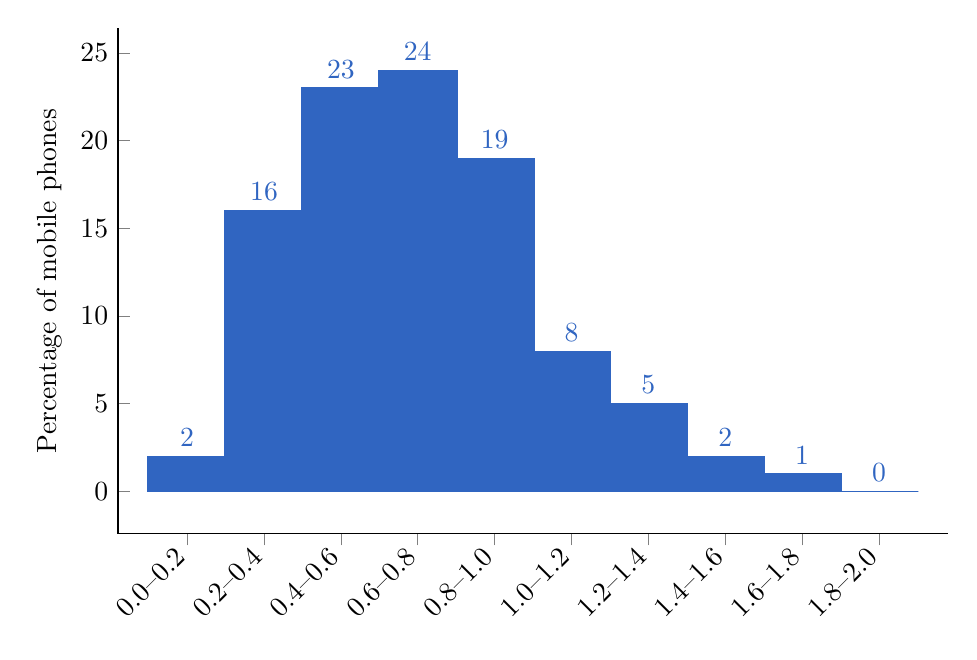
\begin{tikzpicture}
\begin{axis}[
        ybar=-1cm,
        axis x line*=bottom,
        axis y line*=left,
         bar width=1cm,
        height=8cm, width=\textwidth,
        ylabel={Percentage of mobile phones},
        symbolic x coords={0.0--0.2,0.2--0.4,0.4--0.6,0.6--0.8,0.8--1.0,1.0--1.2,1.2--1.4,1.4--1.6,1.6--1.8,1.8--2.0},
        x tick label style={rotate=45, anchor=east, align=left},
        nodes near coords,
        nodes near coords align={vertical}      
        ]
        \addplot[hous,fill]  coordinates {(0.0--0.2,2)};
        \addplot[hous,fill]  coordinates {(0.2--0.4,16)};
        \addplot[hous,fill]  coordinates {(0.4--0.6,23)};
        \addplot[hous,fill]  coordinates {(0.6--0.8,24)};
        \addplot[hous,fill]  coordinates {(0.8--1.0,19)};
        \addplot[hous,fill]  coordinates {(1.0--1.2,8)};
        \addplot[hous,fill]  coordinates {(1.2--1.4,5)};
        \addplot[hous,fill]  coordinates {(1.4--1.6,2)};
        \addplot[hous,fill]  coordinates {(1.6--1.8,1)};
        \addplot[hous,fill]  coordinates {(1.8--2.0,0)};
    \end{axis}
\end{tikzpicture}
todo: xlabel, zeggen dat bovengrens niet inbegrepen is en titel geven.


The $P^{max}_{Tx}$ is for LTE and UMTS 23 Dbm \cite{J11_maxTpxUE, J10_RDP}.

%todo: beslis of je mobile device of UE gaat gebruiken.
To predict the effective transmitted power by the \gls{UE}, the folowing equation is used:

\begin{equation}
P_{Tx} = P_{sens} + PL
\label{eq:calculatesar}
\end{equation}

\begin{equation}
P_{sens} = P_{noise} + SNR - G + IL + NF + IF
\label{eq:calculatepsens}
\end{equation}


\section{Decision Algorithm}

J1 zegt:

The decision for allocating a user to a base sta-
tion is changed. In [19], a base station was only

switched on when there was no active base station
to which the user could connect. This is no longer
the case as discussed in Section 3.2 because this is

not the appropriate decision when optimizing to-
wards exposure.


- prevous model between my "generator" class